\documentclass[11pt,singleside,a4paper,makeidx,notitlepage]{article}
\pdfoutput=1
\usepackage{graphicx}
\usepackage{xspace}
\usepackage{amsmath}
\usepackage{amssymb}
\usepackage{array}
\newcommand{\smodels}{{\tt SModelS}\xspace}
\newcommand{\LL}{\mathcal{L}}
\newcommand{\thetahat}{\hat{\theta}}
\newcommand{\xhat}{\hat{x}}
\newcommand{\muhat}{\hat{\mu}}
\newcommand{\Vb}{{\bf V}}

\newlength{\picwidth}
\setlength{\picwidth}{100pt}
\newlength{\halfwidth}
\setlength{\halfwidth}{170pt}
\newlength{\srh}
\setlength{\srh}{1.2cm}
\newlength{\srl}
\setlength{\srl}{-1.5cm}

\begin{document}
\title{Comparison}
%\section*{Comparison}

\begin{figure}[h!t]
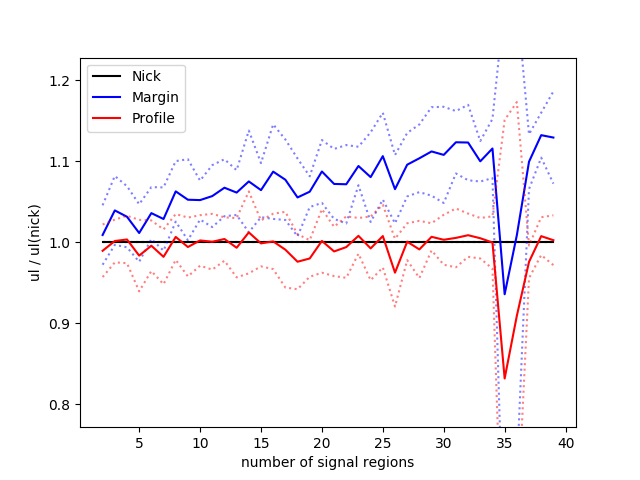
\includegraphics[width=420pt]{comp.png}
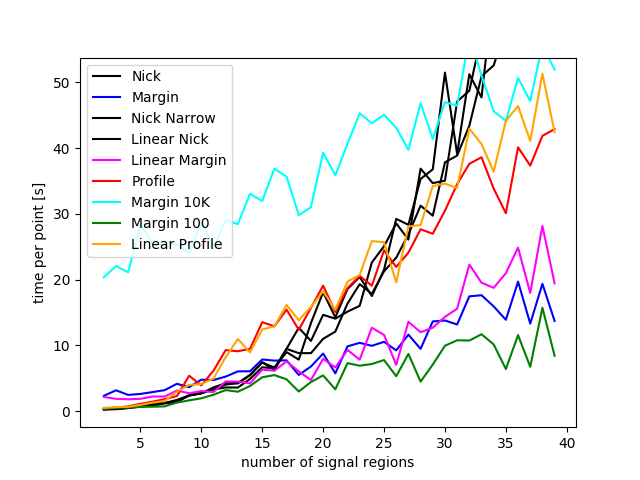
\includegraphics[width=420pt]{t.png}
\caption{Ratios of upper limits (top), CPU time (bottom)}
\end{figure}


\end{document}
